\subsection{Session 2, Exercise 04}

\lineparagraph{Exercise}

Let $\Sigma=\{0,1\}$. Give a deterministic finite automaton that accepts the words that do not contain the subword $001$.

\lineparagraph{Solution}

When dealing with \textbf{deterministic} finite automatons, a useful trick to keep in mind: sometimes it is easier to give a DFA for the complementer of the language, and then a DFA for the original language can be quickly created.

IMPORTANT: This trick only works for \textbf{deterministic finite automatons}!!!

\textbf{Step 1}: Create DFA for the complementer of the language:

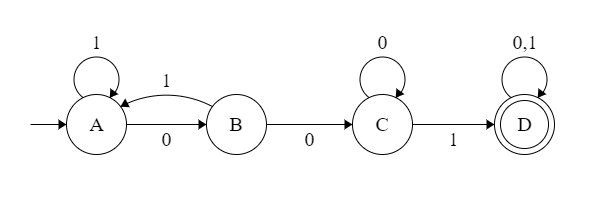
\includegraphics[width=0.6\linewidth]{02/2_4.png}

\textbf{Step 2}: Invert the accept/reject status of the states:

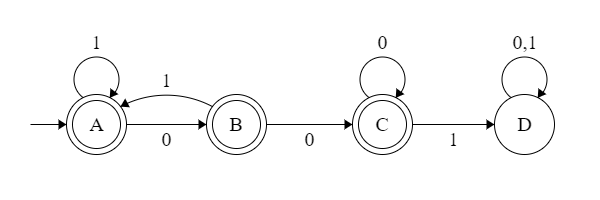
\includegraphics[width=0.6\linewidth]{02/2_4_inv.png}

Proof:

Let's look at what the states mean:

\begin{itemize}
    \item A: State $A$ represents words that end in something that is not a prefix of $001$: they either are the empty string or they end in a $1$; and do not contain $001$ itself.
    \item B: State $B$ represents words that end in $0$.
    \item C: State $C$ represents words that end in $00$.
    \item D: State $D$ represents words that contain $001$.
\end{itemize}

Let's look at the starting state and the accepting and rejecting states:

\begin{itemize}
    \item The starting state is the state that should represent the empty string. The empty string contains no prefix of $001$, so it is represented by $A$.
    \item In the original DFA words that contain $001$ were accepted, which is represented by state $D$, while states $A$,$B$ and $C$ were rejecting.
    \item To get a DFA for the complementer of the language, we simply need to accepts words that we have rejected before and reject words that we have accepted before. This is done by making states $A$,$B$ and $C$ accept, while making state $D$ reject.
\end{itemize}

Let's look at the transitions:

\begin{itemize}
    \item In state $A$, when we read in a $0$ we can move to state $B$, since now the current ending is $0$. However when we read $1$'s, we are not getting closer to finding a $001$ substring (we need the $0$'s first), so we just discard them.
    \item In state $B$, we have the ending $0$. When we read another $0$ in, this results in having the ending $00$, so we can move forward to state $C$, one step closer to finding the substring $001$. However if we read in a $1$, this ruins our progress, since the current ending is now $01$, but we needed a $00$. We can't even stay in state $B$, since we would need a $0$ ending for that, but the last character has been a $1$. We have to move all the way back to state $A$.
    \item In state $C$ the current ending is $00$. If we read in a $1$, that means we just found a $001$ substring, we can move to state $D$! And if we read a $0$ in, while we can't move to state $D$, we can stay in $C$, since the current ending is $000$, or discarding the oldest $0$: $00$, which means we can stay in state $C$.
    \item In state $D$ we have already found the substring, we just read in the remainder of the input, discard it and accept when done.
\end{itemize}